\documentclass[12pt,a4paper]{article}

\usepackage[T1]{fontenc}
\usepackage[utf8]{inputenc}
\usepackage[slovak]{babel}
\usepackage{geometry}
\usepackage{graphicx}
\usepackage{float}
\usepackage{booktabs}
\usepackage{tabularx}
\usepackage{hyperref}
\usepackage{enumitem}
\usepackage{tikz} %for graphs
\usetikzlibrary{arrows.meta, positioning, shapes.geometric}

\geometry{margin=2.5cm}
\graphicspath{{../schemy/}}

\title{Riadenie prevádzky veternej elektrárne\\Princípy informačných systémov}
\author{Kačmárová Lucia \and meno1 \and meno2}
\date{Akademický rok 2025/2026}

\begin{document}

\hypersetup{pageanchor=false}
\begin{titlepage}
  \centering
  {\Large Slovenská technická univerzita v Bratislave\par}
  {\Large Fakulta informatiky a informačných technológií\par}
  \vspace{3cm}
  {\huge\bfseries Riadenie prevádzky veternej elektrárne\par}
  \vspace{0.5cm}
  {\Large Princípy informačných systémov\par}
  \vspace{2.5cm}

  {\large Kačmárová Lucia, Múdry Filip, Podolan Šimon\par}
  \vfill

  \begin{tabular}{rl}
    Cvičenie: & Štvrtok, 9:00 \\
    Cvičiaci: & Ádám Kemény \\
    Akademický rok: & 2025/2026 \\
  \end{tabular}
\end{titlepage}
\hypersetup{pageanchor=true}

\tableofcontents
\newpage

\section{Rámcová téma}
Téma projektu je zameraná na riadenie prevádzky veternej elektrárne, konkrétne na procesy spojené so spustením výroby elektriny, jej monitorovaním a riešením porúch. Veterná elektráreň je komplexný systém, ktorý zahŕňa automatizované riadiace prvky aj ľudské zásahy. Cieľom je zabezpečiť bezpečnú a stabilnú výrobu elektrickej energie v závislosti od aktuálnych podmienok. V rámci tejto témy boli identifikované tri hlavné procesy:

\begin{enumerate}
  \item \textbf{Spustenie výroby elektriny}
  \item \textbf{Monitorovanie a regulácia prevádzky}
  \item \textbf{Riešenie poruchy a obnovenie prevádzky}
\end{enumerate}


\section*{Použité skratky rolí}
\noindent
\begin{tabular}{@{}>{\bfseries}l p{0.8\textwidth}}
RS   & Riadiaci systém  \\
DDS & Dispečer distribučnej siete \\
O  & Operátor elektrárne \\
ST  & Servisný technik \\
\end{tabular}





%%%%%%%%%%%%%%%%%%%%%%%%%%%%%%%%%%%%%%%%%%%%%%%%%%%%%%%%%%%%%%
%P1
%%%%%%%%%%%%%%%%%%%%%%%%%%%%%%%%%%%%%%%%%%%%%%%%%%%%%%%%%%%%%%
\newpage
\section{Proces 1 -- Spustenie výroby elektriny}
\subsection{Popis procesu}
Proces spustenia výroby elektriny začína inicializáciou spúšťacej procedúry v riadiacom systéme. Po iniciálnom signáli RS najprv získa aktuálne údaje o poveternostných podmienkach (predovšetkým o rýchlosti a smere vetra) z meteorologických senzorov inštalovaných na veternej elektrárni. Následne získa krátkodobú predpoveď zo služby poveternostných údajov, aby mal kompletný obraz nielen o aktuálnom stave, ale aj o predpokladanom vývoji počasia. Na základe získaných údajov RS vyhodnotí, či sú poveternostné podmienky vhodné pre spustenie výroby (vyhodnocuje sa najmä minimálna a maximálna prípustná rýchlosť vetra). Ak podmienky nie sú splnené (príliš slabý alebo príliš silný vietor), proces sa ukončí bez spustenia výroby. Ak sú podmienky vyhovujúce, proces pokračuje kontrolou technického stavu turbíny, čiže RS overuje funkčnosť hlavných komponentov ako lopatky, generátor, brzdný systém a senzory.

\vspace{0.6em}
Po úspešnej kontrole technického stavu RS paralelne spúšťa dve kontroly:
\begin{enumerate}[noitemsep, topsep=2pt, leftmargin=1.5cm]
    \item \textbf{kontrolu bezpečnostných limitov} (vibrácie, teploty, hraničné hodnoty)
    \item \textbf{overenie pripojenia do distribučnej siete}, ktoré vykonáva DDS
\end{enumerate}
\vspace{0.6em}
Po dokončení oboch paralelných kontrol RS vyžiada od DDS finálne povolenie pripojenia. DDS na základe stavu siete buď povolenie udelí, zamietne (napr. pri nedostatočnej kapacite), alebo nereaguje v stanovenom časovom okne, a vtedy RS vyhodnotí timeout. V prípade zamietnutia alebo timeoutu sa proces ukončí.Po udelení povolenia RS pristupuje k samotnému nastaveniu turbíny. Paralelne vykonáva tri činnosti: natočenie gondoly do správneho smeru voči vetru, nastavenie uhla lopatiek (pitch) a spustenie pomocných systémov (chladenie, mazanie, riadiaca elektronika). Po dokončení všetkých troch nastavení je turbína pripravená a RS spustí generátor. Po spustení nasleduje ramp-up výkonu, čo je postupné nábehové zvyšovanie produkcie energie. Posledným krokom je manuálne potvrdenie úspešného spustenia výroby operátorom elektrárne. Proces sa končí stavom \textbf{Výroba spustená} a nadväzuje na proces monitorovania a regulácie prevádzky.






%%%%%%%%%%%%%%%%%%%%%%%%%%%%%%%%%%%%%%%%%%%%%%%%%%%%%%%%%%%%%%
%Process info
%%%%%%%%%%%%%%%%%%%%%%%%%%%%%%%%%%%%%%%%%%%%%%%%%%%%%%%%%%%%%%
\subsection{Procesné informácie (tokeny, prechody, stavy)}
\begin{table}[H]
  \centering
  \renewcommand{\arraystretch}{1.2}
  \begin{tabularx}{\textwidth}{|p{0.22\textwidth}|X|}
    \hline
    \textbf{Názov procesu} & Spustenie výroby elektriny \\
    \hline
    \textbf{Popis} & Po inicializácii RS získa údaje o vetre a predpoveď, vyhodnotí poveternostné podmienky, vykoná kontrolu technického stavu, paralelne overí bezpečnostné limity a pripojenie do siete (DDS), vyžiada povolenie pripojenia od DDS, paralelne nastaví turbínu (gondola, lopatky, pomocné systémy), spustí generátor a operátor potvrdí spustenie. \\
    \hline
    \textbf{Roly} & RS, O, DDS \\
    \hline
    \textbf{Vstupné tokeny} & Iniciálny signál spustenia (1 token v P0), meteorologické údaje, status komponentov, informácia o dostupnosti pripojenia \\
    \hline
    \textbf{Výstupné tokeny} & \textbf{Výroba spustená} (úspech), alebo \textbf{Proces ukončený} pri: nevyhovujúcich podmienkach / zamietnutom povolení / timeoute \\
    \hline
    \textbf{Prechody (22)} & Získaj údaje o vetre, Získaj predpoveď, Vyhodnoť podmienky, Podmienky nesplnené, Podmienky splnené, Skontroluj technický stav, Spusti prípravu (AND split), Skontroluj bezpečnostné limity, Over pripojenie do siete, Kontroly dokončené (AND join), Vyžiadaj povolenie pripojenia, Povolenie udelené, Povolenie zamietnuté, Timeout odpovede, Nastav turbínu (AND split), Natoč gondolu, Nastav uhol lopatiek, Spusť pomocné systémy, Turbína pripravená (AND join), Spusť generátor, Ramp-up výkonu, Potvrď spustenie výroby \\
    \hline
    \textbf{Stavy (15)} & Spustenie iniciované, Údaje o vetre získané, Predpoveď získaná, Podmienky vyhodnotené, Pokračuj v kontrole, Technický stav OK, Bezpečnosť OK, Pripojenie OK, Kontroly dokončené, Čaká sa na povolenie, Povolenie udelené, Turbína pripravená, Generátor spustený, Výkon nabieha, Výroba spustená \\
    \hline
  \end{tabularx}
  \caption{Proces 1 -- Zhrnutie procesu}
\end{table}



%%%%%%%%%%%%%%%%%%%%%%%%%%%%%%%%%%%%%%%%%%%%%%%%%%%%%%%%%%%%%%
%Roles 
%%%%%%%%%%%%%%%%%%%%%%%%%%%%%%%%%%%%%%%%%%%%%%%%%%%%%%%%%%%%%%
\subsection{Procesné roly}
\begin{table}[H]
  \centering
  \renewcommand{\arraystretch}{1.2}
  \begin{tabularx}{\textwidth}{|p{0.22\textwidth}|X|}
    \hline
    \textbf{Rola} & \textbf{Úloha} \\
    \hline
    RS & Automatizovaný riadiaci subsystém veternej elektrárne. Zbiera meteorologické údaje a predpoveď, vyhodnocuje poveternostné podmienky, vykonáva kontroly technického stavu a bezpečnostných limitov, vyžaduje povolenie od DDS, vyhodnocuje timeout odpovede a po udelení povolenia paralelne nastavuje turbínu (gondola, lopatky, pomocné systémy), spúšťa generátor a riadi ramp-up výkonu. \\
    \hline
    O & Manuálne potvrdzuje úspešné spustenie výroby ako finálny krok procesu. Vykonáva dohľad nad celým procesom a v prípade neštandardných situácií môže zasiahnuť (napr. manuálne zrušiť spustenie). \\
    \hline
    DDS & Overuje stav distribučnej siete a jej kapacitu. Udeľuje alebo zamieta povolenie na pripojenie elektrárne do siete na základe aktuálnych podmienok v sieti. \\
    \hline
  \end{tabularx}
  \caption{Proces 1 -- Popis rolí}
\end{table}



%%%%%%%%%%%%%%%%%%%%%%%%%%%%%%%%%%%%%%%%%%%%%%%%%%%%%%%%%%%%%%
%Roles & activities
%%%%%%%%%%%%%%%%%%%%%%%%%%%%%%%%%%%%%%%%%%%%%%%%%%%%%%%%%%%%%%
\subsection{Procesné roly (priradenie činností)}
\begin{table}[H]
  \centering
  \small
  \renewcommand{\arraystretch}{1.2}
  \begin{tabularx}{\textwidth}{|l|X|c|c|c|}
    \hline
    \textbf{ID} & \textbf{Činnosť (prechod)} & \textbf{RS} & \textbf{O} & \textbf{DDS} \\
    \hline
    t1 & Získaj údaje o vetre & X & & \\ \hline
    t2 & Získaj predpoveď & X & & \\ \hline
    t3 & Vyhodnoť podmienky & X & & \\ \hline
    t4 & Podmienky nesplnené & X & & \\ \hline
    t5 & Podmienky splnené & X & & \\ \hline
    t6 & Skontroluj technický stav & X & & \\ \hline
    t7 & Spusti prípravu (AND split) & X & & \\ \hline
    t8 & Skontroluj bezpečnostné limity & X & & \\ \hline
    t9 & Over pripojenie do siete & & & X \\ \hline
    t10 & Kontroly dokončené (AND join) & X & & \\ \hline
    t11 & Vyžiadaj povolenie pripojenia & X & & \\ \hline
    t12 & Povolenie udelené & & & X \\ \hline
    t13 & Povolenie zamietnuté & & & X \\ \hline
    t14 & Timeout odpovede & X & & \\ \hline
    t15 & Nastav turbínu (AND split) & X & & \\ \hline
    t16 & Natoč gondolu & X & & \\ \hline
    t17 & Nastav uhol lopatiek & X & & \\ \hline
    t18 & Spusť pomocné systémy & X & & \\ \hline
    t19 & Turbína pripravená (AND join) & X & & \\ \hline
    t20 & Spusť generátor & X & & \\ \hline
    t21 & Ramp-up výkonu & X & & \\ \hline
    t22 & Potvrď spustenie výroby & & X & \\ \hline
  \end{tabularx}
  \caption{Proces 1 -- Priradenie činností k rolám}
\end{table}


%%%%%%%%%%%%%%%%%%%%%%%%%%%%%%%%%%%%%%%%%%%%%%%%%%%%%%%%%%%%%%
%Petri net
%%%%%%%%%%%%%%%%%%%%%%%%%%%%%%%%%%%%%%%%%%%%%%%%%%%%%%%%%%%%%%
\subsection{Petriho sieť}
Navrhnutý model Petriho siete reprezentuje sekvenčno-paralelnú logiku riadenia procesu. Obsahuje mechanizmy vetvenia typu \textbf{XOR} pre rozhodovacie procesy (napr. kontrola podmienok alebo udelenie povolenia) a \textbf{AND} pre paralelné vykonávanie úloh (technické kontroly a nastavovanie turbíny).

\begin{figure}[H]
  \hspace*{-2cm}
  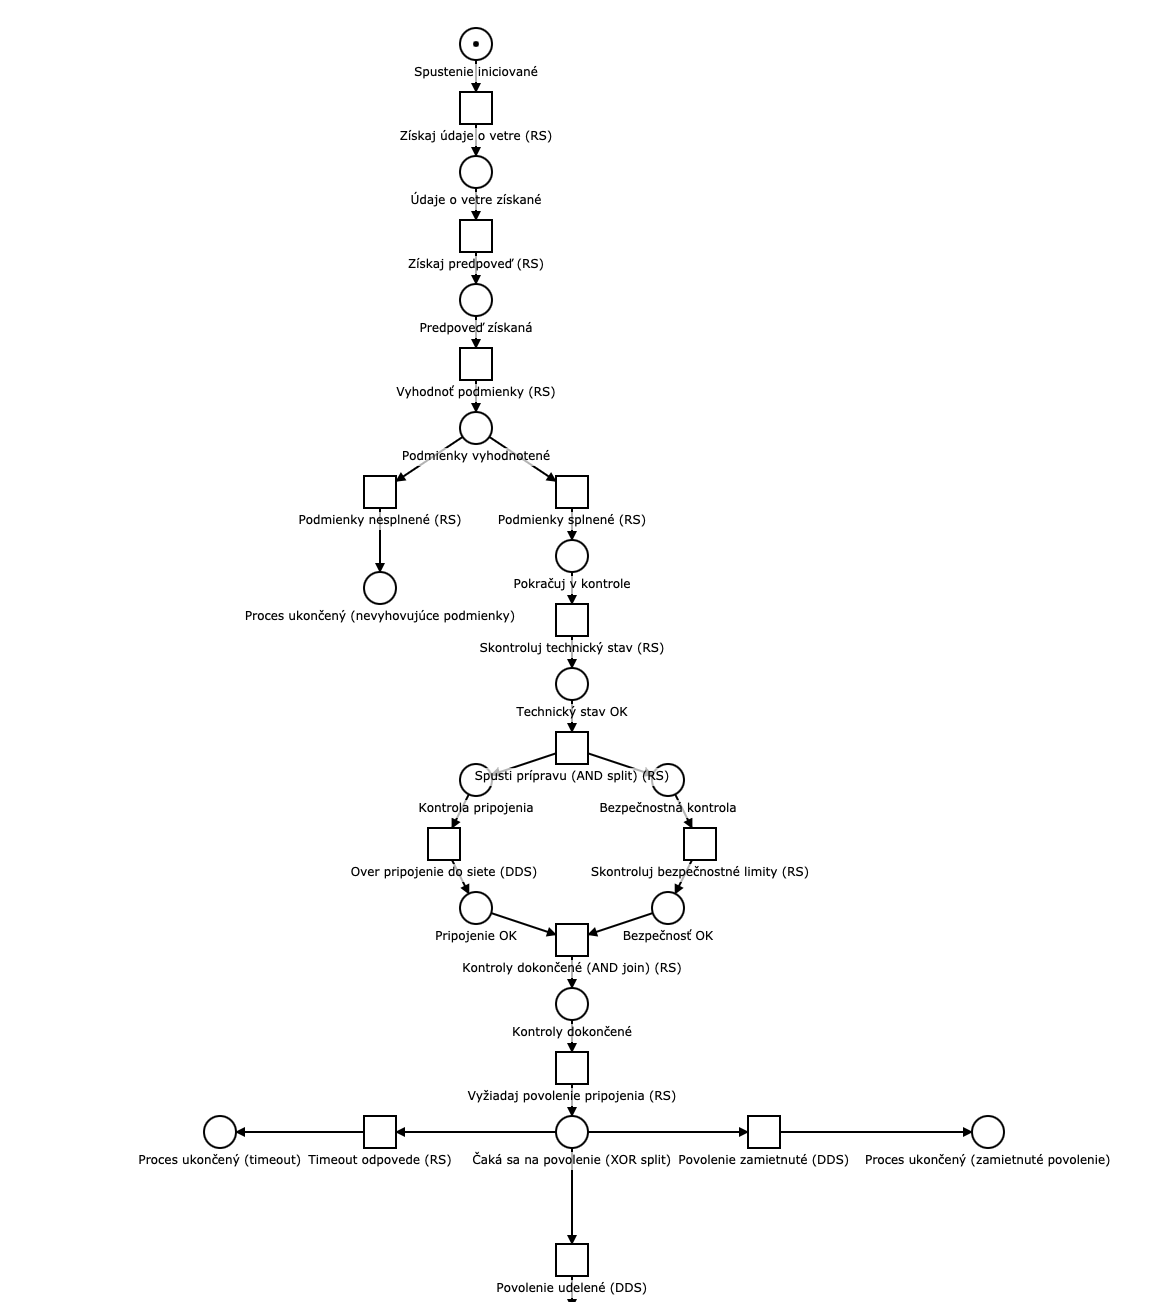
\includegraphics[width=1.2\textwidth]{figs/P1/PS_P1_1.png}
  \caption{Petriho sieť pre Proces 1 (časť 1)}
\end{figure}

\begin{figure}[H]
  \hspace*{-2cm}
  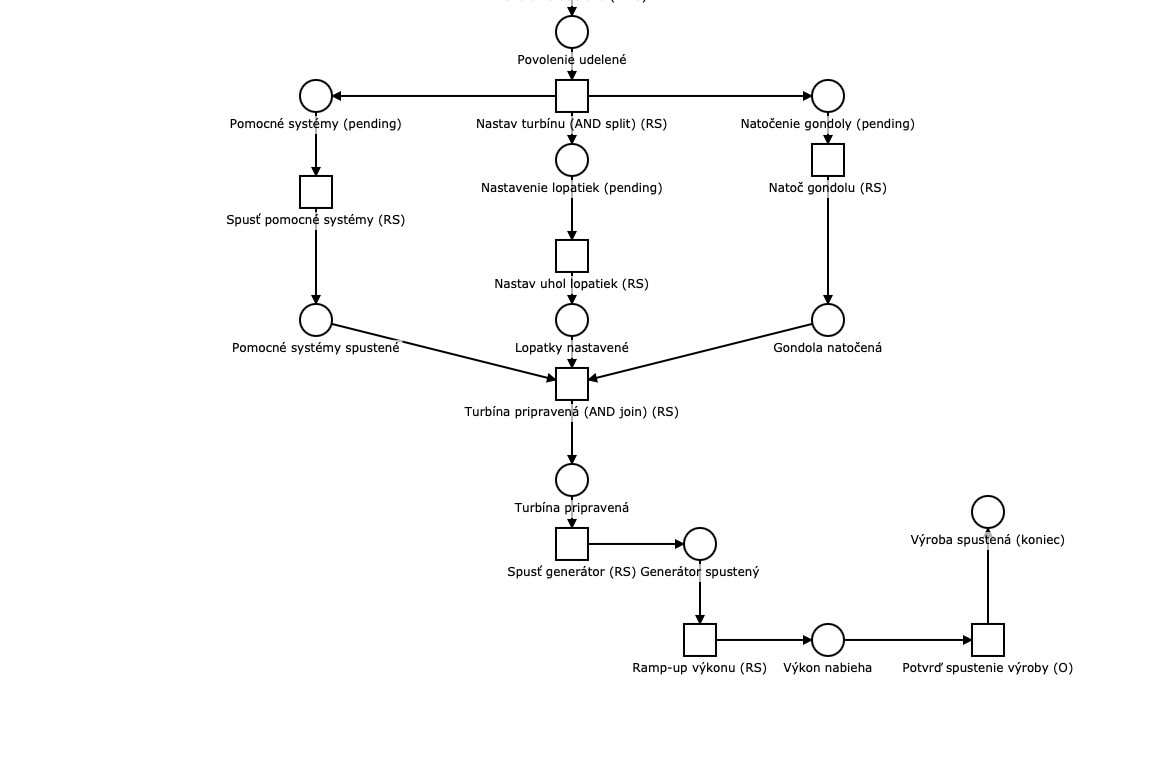
\includegraphics[width=1.2\textwidth]{figs/P1/PS_P1_2.png}
  \caption{Petriho sieť pre Proces 1 (časť 2)}
\end{figure}


%%%%%%%%%%%%%%%%%%%%%%%%%%%%%%%%%%%%%%%%%%%%%%%%%%%%%%%%%%%%%%
%Reachability graph
%%%%%%%%%%%%%%%%%%%%%%%%%%%%%%%%%%%%%%%%%%%%%%%%%%%%%%%%%%%%%%
\newpage
\subsection{Graf dosiahnuteľnosti}
\begin{figure}[H]
  \centering
  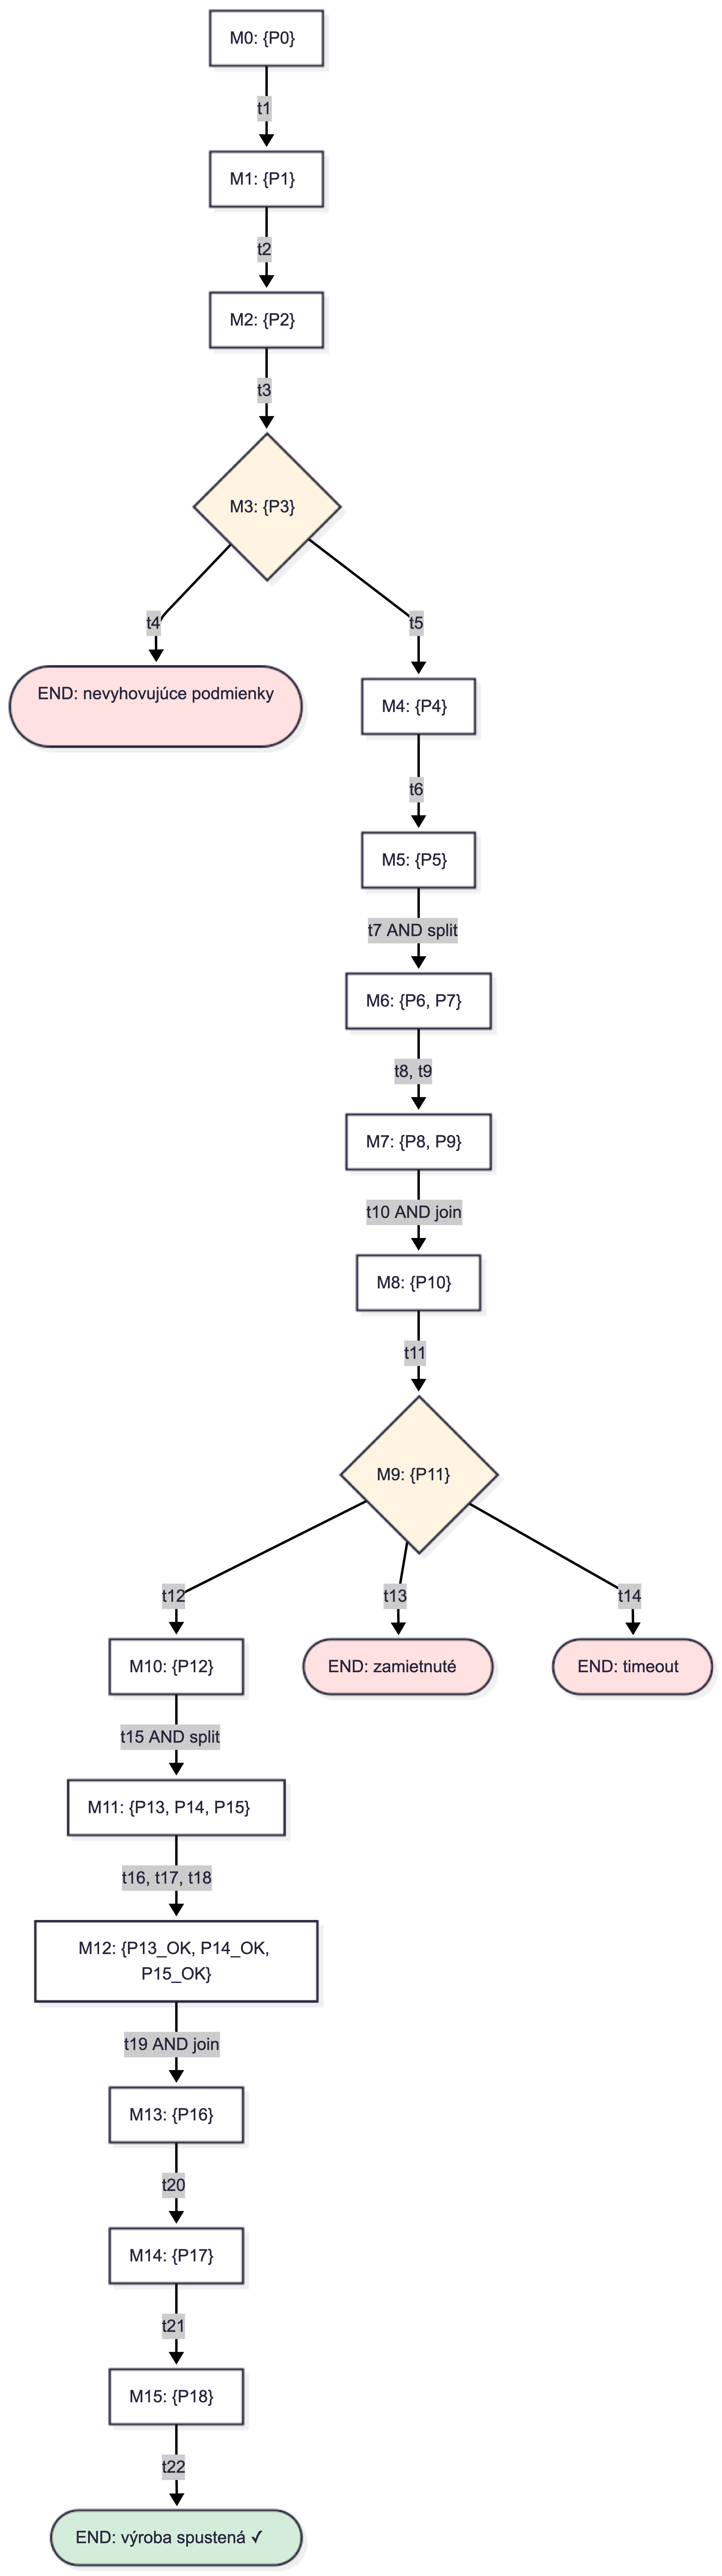
\includegraphics[height=0.9\textheight]{figs/P1/P1_ReachabilityGraph.png}
  \caption{Proces 1 -- Graf dosiahnuteľnosti}
\end{figure}


%%%%%%%%%%%%%%%%%%%%%%%%%%%%%%%%%%%%%%%%%%%%%%%%
%Screens
%%%%%%%%%%%%%%%%%%%%%%%%%%%%%%%%%%%%%%%%%%%%%%%%
\newpage
\subsection{Obrazovky}
\emph{TODO: Doplniť}



%%%%%%%%%%%%%%%%%%%%%%%%%%%%%%%%%%%%%%%%%%%%%%%%
%BPMN's
%%%%%%%%%%%%%%%%%%%%%%%%%%%%%%%%%%%%%%%%%%%%%%%%
\newpage
\subsection{BPMN}
\begin{figure}[H]
  \centering
  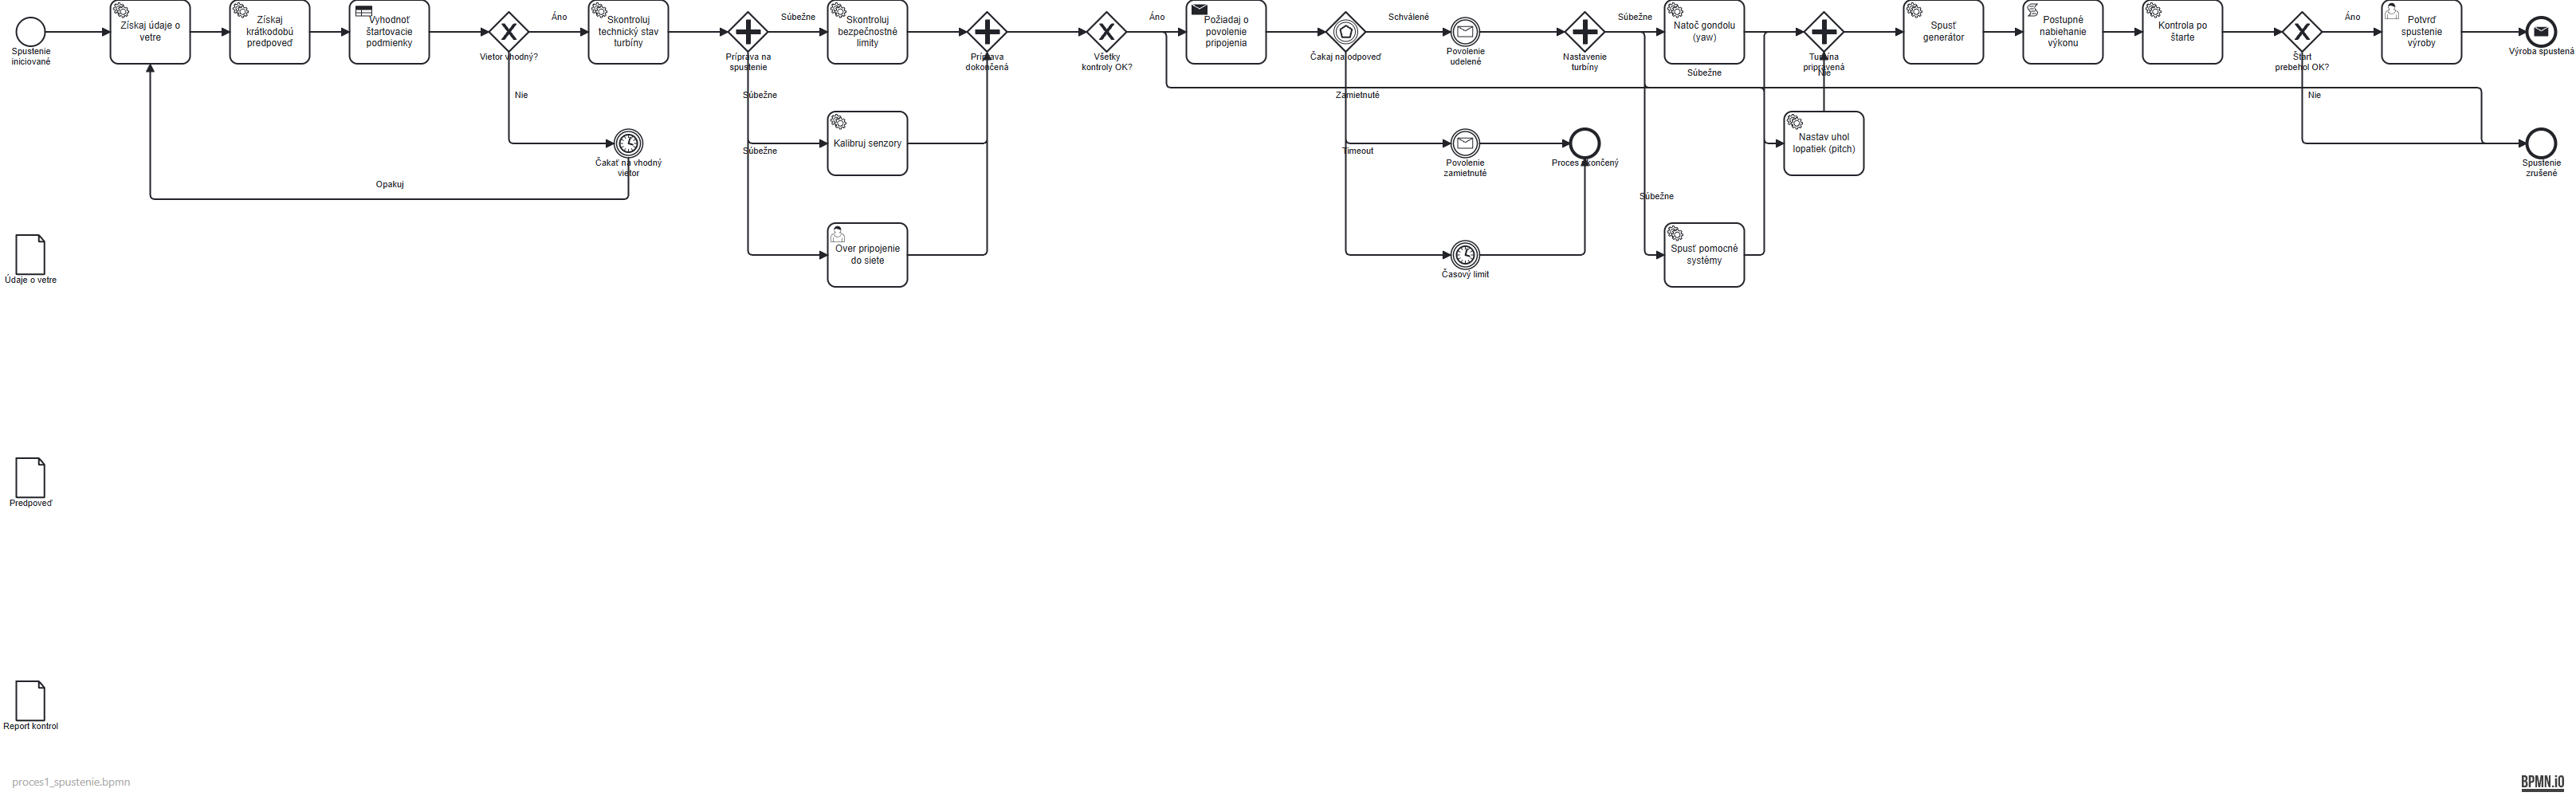
\includegraphics[width=\textwidth]{figs/P1/proces1-spustenie.png}
  \caption{Proces 1 -- BPMN model}
\end{figure}











%%%%%%%%%%%%%%%%%%%%%%%%%%%%%%%%%%%%%%%%%%%%%%%%%%%%%%%%%%%%%%
%P2
%%%%%%%%%%%%%%%%%%%%%%%%%%%%%%%%%%%%%%%%%%%%%%%%%%%%%%%%%%%%%%
\newpage
\section{Proces 2 -- Monitorovanie a regulácia prevádzky}
\subsection{Popis procesu}
Proces monitorovania a regulácie prevádzky začína ihneď po úspešnom spustení výroby elektriny. Riadiaci systém (RS) priebežne zbiera senzorové dáta a predspracúva ich pre ďalšie vyhodnotenie. Následne paralelne monitoruje dve skupiny parametrov: 
\vspace{0.6em}
\begin{enumerate}[noitemsep, topsep=2pt, leftmargin=1.5cm]
    \item \textbf{rýchlosť vetra a výkon generátora na jednej strane}
    \item \textbf{teploty a vibrácie komponentov na druhej strane}
\end{enumerate}
\vspace{0.6em}
Po dokončení oboch monitorovacích vetiev RS čaká na jednu z troch udalostí:
\vspace{0.6em}
\begin{enumerate}[noitemsep, topsep=2pt, leftmargin=1.5cm]
    \item \textbf{Uplynul pravidelný časový interval}
    \item \textbf{RS detegoval alarm alebo odchýlku}
     \item \textbf{DDS zaslal požiadavku na reguláciu výkonu}
\end{enumerate}
\vspace{0.6em}

Ak udalosťou je uplynulý interval alebo alarm, RS vyhodnotí údaje a rozhodne o stave prevádzky. Pri stabilnej prevádzke RS vypočíta optimálne nastavenia a paralelne ich aplikuje na tri subsystémy: pitch lopatiek, yaw gondoly a menič/brzdový systém. Po dokončení nastavení RS overí bezpečnostné limity. Ak sú limity v poriadku, DDS dostane údaje o výrobe, zaeviduje ich a proces pokračuje ďalším monitorovacím cyklom. Ak limity nie sú v poriadku, je vyžiadaný zásah operátora.
Pri nestabilnej prevádzke RS klasifikuje závažnosť odchýlky. V prípade menšej odchýlky je vyžiadaný zásah operátora elektrárne (O), kde operátor preskúma odchýlku a rozhodne, či je potrebná fyzická kontrola turbíny. Fyzická kontrola sa vykoná alebo sa preskočí, následne operátor upraví parametre, RS aplikuje a zaznamená zmeny a proces sa vracia do monitorovacieho cyklu. V prípade závažnej odchýlky alebo poruchy RS aktivuje prechod na Proces 3 (Riešenie poruchy).
Ak udalosťou je požiadavka DDS na reguláciu, operátor potvrdí požiadavku, RS upraví setpoint výkonu, DDS dostane potvrdenie a zaeviduje reguláciu, a proces sa vracia do monitorovacieho cyklu. Proces je cyklický a beží kontinuálne po celú dobu prevádzky elektrárne.






%%%%%%%%%%%%%%%%%%%%%%%%%%%%%%%%%%%%%%%%%%%%%%%%%%%%%%%%%%%%%%
%Process info
%%%%%%%%%%%%%%%%%%%%%%%%%%%%%%%%%%%%%%%%%%%%%%%%%%%%%%%%%%%%%%
\noindent
\subsection{Procesné informácie (tokeny, prechody, stavy)}
\begin{table}[H]
  \centering
  \renewcommand{\arraystretch}{1.2}
  \begin{tabularx}{\textwidth}{|p{0.22\textwidth}|X|}
    \hline
    \textbf{Názov procesu} & Monitorovanie a regulácia prevádzky \\
    \hline
    \textbf{Popis} & RS priebežne zbiera a predspracúva senzorové dáta, paralelne monitoruje prevádzkové parametre a čaká na udalosť. Pri stabilnej prevádzke paralelne optimalizuje nastavenia (pitch, yaw, menič), overí limity a odošle údaje DDS. Pri nestabilnej prevádzke klasifikuje odchýlku, menšia vedie k zásahu operátora a úprave parametrov, závažná k prechodu na Proces 3. Požiadavka DDS na reguláciu vedie k samostatnej vetve, kde O potvrdí zmenu, RS upraví setpoint a DDS zaeviduje reguláciu. Proces je cyklický. \\
    \hline
    \textbf{Roly} & RS, O, DDS \\
    \hline
    \textbf{Vstupné tokeny} & 1 token v P0, priebežné merania zo senzorov, alarmy, požiadavky DDS \\
    \hline
    \textbf{Výstupné tokeny} & Odoslané a zaevidované údaje o výrobe, upravené prevádzkové parametre, alebo token v P\_TO\_TROUBLE (prechod na P3) \\
    \hline
    \textbf{Prechody (42)} & Zbieraj senzorové dáta, Predspracuj dáta, Paralelné monitorovanie, Sleduj vietor a výkon, Sleduj teploty a vibrácie, Monitorovanie dokončené, Uplynul interval, Alarm/odchýlka detegovaná, Požiadavka DDS na reguláciu, Vyhodnoť údaje, Stabilná prevádzka, Nestabilná prevádzka, Vypočítaj optimálne nastavenia, Aplikuj nastavenia, Nastav pitch, Nastav yaw, Nastav menič/brzdy, Nastavenia aplikované, Over bezpečnostné limity, Limity OK, Limity NIE, Odošli údaje o výrobe, Zaeviduj údaje v sieti, Ďalší cyklus, Vyžiadaj zásah operátora, Preskúmaj odchýlku, Fyzická kontrola potrebná, Fyzická kontrola netreba, Fyzická kontrola turbíny, Uprav parametre, Aplikuj zmeny, Zaznamenaj zmeny, Späť na monitoring, Klasifikuj odchýlku, Menšia odchýlka, Závažná odchýlka, Prechod na riešenie poruchy, Potvrď požiadavku DDS, Uprav setpoint výkonu, Odošli potvrdenie DDS, Zaeviduj reguláciu, Späť na monitoring \\
    \hline
    \textbf{Stavy (41)} & Monitoring aktívny, Dáta zozbierané, Dáta predspracované, Vietor/výkon, Teploty/vibrácie, Vietor/výkon vyhodnotené, Teploty/vibrácie vyhodnotené, Čakaj na udalosť, Spusti vyhodnotenie, Údaje vyhodnotené, Stabilná prevádzka, Nestabilita detegovaná, Nastavenia vypočítané, Pitch/Yaw/Menič, Pitch/Yaw/Menič nastavené, Nastavenia aplikované, Limity skontrolované, Limity OK, Limity NIE, Údaje odoslané, Údaje zaevidované, Operátor informovaný, Odchýlka preskúmaná, Fyzická kontrola vykonaná, Bez fyzickej kontroly, Parametre upravené, Zmeny aplikované, Zmeny zaznamenané, Odchýlka klasifikovaná, Menšia odchýlka, Závažná odchýlka, Regulácia potvrdená, Setpoint upravený, Potvrdenie odoslané, Regulácia zaevidovaná, Prechod na riešenie poruchy \\
    \hline
  \end{tabularx}
  \caption{Proces 2 -- Zhrnutie procesu}
\end{table}




%%%%%%%%%%%%%%%%%%%%%%%%%%%%%%%%%%%%%%%%%%%%%%%%%%%%%%%%%%%%%%
%Roles
%%%%%%%%%%%%%%%%%%%%%%%%%%%%%%%%%%%%%%%%%%%%%%%%%%%%%%%%%%%%%%
\subsection{Procesné roly}
\begin{table}[H]
  \centering
  \renewcommand{\arraystretch}{1.2}
  \begin{tabularx}{\textwidth}{|p{0.22\textwidth}|X|}
    \hline
    \textbf{Rola} & \textbf{Úloha} \\
    \hline
    RS & Zbiera a predspracúva senzorové dáta, paralelne monitoruje
    prevádzkové parametre (vietor/výkon a teploty/vibrácie), vyhodnocuje stabilitu
    prevádzky, počíta a paralelne aplikuje optimálne nastavenia (pitch, yaw,
    menič/brzdy), overuje bezpečnostné limity, klasifikuje závažnosť odchýlok,
    vyžiada zásah operátora pri nestabilite, aplikuje a zaznamenáva zmeny
    parametrov, upravuje setpoint výkonu pri požiadavke DDS a zabezpečuje
    návrat do monitorovacieho cyklu. Pri závažnej poruche aktivuje prechod
    na Proces~3. \\
    \hline
    O & Preskúmava odchýlky a rozhoduje o potrebe fyzickej
    kontroly turbíny. Vykonáva fyzickú kontrolu a upravuje prevádzkové parametre.
    Potvrdzuje požiadavky DDS na reguláciu výkonu. \\
    \hline
    DDS & Posiela požiadavky na reguláciu výkonu podľa
    aktuálnej situácie v distribučnej sieti. Prijíma a eviduje údaje o výrobe
    elektriny a potvrdenia o vykonanej regulácii. \\
    \hline
  \end{tabularx}
  \caption{Proces 2 -- Popis rolí}
\end{table}



%%%%%%%%%%%%%%%%%%%%%%%%%%%%%%%%%%%%%%%%%%%%%%%%%%%%%%%%%%%%%%
%Roles & activities
%%%%%%%%%%%%%%%%%%%%%%%%%%%%%%%%%%%%%%%%%%%%%%%%%%%%%%%%%%%%%%
\subsection{Procesné roly (priradenie činností)}
\begin{table}[H]
  \centering
  \small
  \renewcommand{\arraystretch}{1.2}
  \begin{tabularx}{\textwidth}{|X|p{0.12\textwidth}|p{0.12\textwidth}|p{0.12\textwidth}|}
    \hline
    \textbf{Činnosť} & \textbf{RS} & \textbf{O} & \textbf{DDS} \\
    \hline
    Zbieraj senzorové dáta & X & & \\
    \hline
    Predspracuj dáta & X & & \\
    \hline
    Paralelné monitorovanie (AND split) & X & & \\
    \hline
    Sleduj vietor a výkon & X & & \\
    \hline
    Sleduj teploty a vibrácie & X & & \\
    \hline
    Monitorovanie dokončené (AND join) & X & & \\
    \hline
    Zachyť udalosť -- interval & X & & \\
    \hline
    Zachyť udalosť -- alarm & X & & \\
    \hline
    Požiadavka DDS na reguláciu & & & X \\
    \hline
    Vyhodnoť údaje & X & & \\
    \hline
    Stabilná prevádzka & X & & \\
    \hline
    Nestabilná prevádzka & X & & \\
    \hline
    Vypočítaj optimálne nastavenia & X & & \\
    \hline
    Aplikuj nastavenia (AND split) & X & & \\
    \hline
    Nastav pitch & X & & \\
    \hline
    Nastav yaw & X & & \\
    \hline
    Nastav menič/brzdy & X & & \\
    \hline
    Nastavenia aplikované (AND join) & X & & \\
    \hline
    Over bezpečnostné limity & X & & \\
    \hline
    Limity OK & X & & \\
    \hline
    Limity NIE & X & & \\
    \hline
    Odošli údaje o výrobe & & & X \\
    \hline
    Zaeviduj údaje v sieti & & & X \\
    \hline
    Ďalší cyklus & X & & \\
    \hline
    Klasifikuj odchýlku & X & & \\
    \hline
    Menšia odchýlka & X & & \\
    \hline
    Závažná odchýlka & X & & \\
    \hline
    Vyžiadaj zásah operátora & X & & \\
    \hline
    Preskúmaj odchýlku & & X & \\
    \hline
    Fyzická kontrola potrebná & & X & \\
    \hline
    Fyzická kontrola netreba & & X & \\
    \hline
    Fyzická kontrola turbíny & & X & \\
    \hline
    Uprav prevádzkové parametre & & X & \\
    \hline
    Aplikuj zmeny v systéme & X & & \\
    \hline
    Zaznamenaj zmeny & X & & \\
    \hline
    Späť na monitoring & X & & \\
    \hline
    Prechod na riešenie poruchy & X & & \\
    \hline
  \end{tabularx}
  \caption{Proces 2 -- Priradenie činností k rolám (časť 1)}
\end{table}

\begin{table}[H]
  \centering
  \small
  \renewcommand{\arraystretch}{1.2}
  \begin{tabularx}{\textwidth}{|X|p{0.12\textwidth}|p{0.12\textwidth}|p{0.12\textwidth}|}
    \hline
    \textbf{Činnosť} & \textbf{RS} & \textbf{O} & \textbf{DDS} \\
    \hline
     Potvrď požiadavku DDS & & X & \\
    \hline
    Uprav setpoint výkonu & X & & \\
    \hline
    Odošli potvrdenie DDS & & & X \\
    \hline
    Zaeviduj reguláciu v sieti & & & X \\
    \hline
    Späť na monitoring (DDS vetva) & X & & \\
    \hline
  \end{tabularx}
  \caption{Proces 2 -- Priradenie činností k rolám  (časť 2)}
\end{table}


%%%%%%%%%%%%%%%%%%%%%%%%%%%%%%%%%%%%%%%%%%%%%%%%%%%%%%%%%%%%%%
%Petri net
%%%%%%%%%%%%%%%%%%%%%%%%%%%%%%%%%%%%%%%%%%%%%%%%%%%%%%%%%%%%%%
\newpage
\subsection{Petriho sieť}
Model obsahuje viacero rozhodovaní (XOR split): event-based rozhodovanie
medzi časovým intervalom, alarmom a požiadavkou DDS; rozhodovanie
o stabilite prevádzky; klasifikáciu závažnosti odchýlky; rozhodovanie
o fyzickej kontrole turbíny a overenie bezpečnostných limitov.
Paralelné vetvenie (AND split) je použité dvojnásobne. Pri paralelnom
monitorovaní prevádzkových parametrov (vietor/výkon a teploty/vibrácie)
a pri paralelnej aplikácii nastavení (pitch, yaw, menič/brzdy).
Proces je cyklický, čiže po každom úspešnom cykle sa vracia do stavu
monitorovania. 

Model obsahuje dátové pole typu \textit{multichoice\_map}
(Klasifikácia odchýlky) a \textit{TaskRef} referencujúci úlohu:
\textbf{Deteguj poruchu (RS)} z Procesu~3, čím je zabezpečené prepojenie procesov pri závažnej poruche.

\begin{figure}[H]
  \centering
  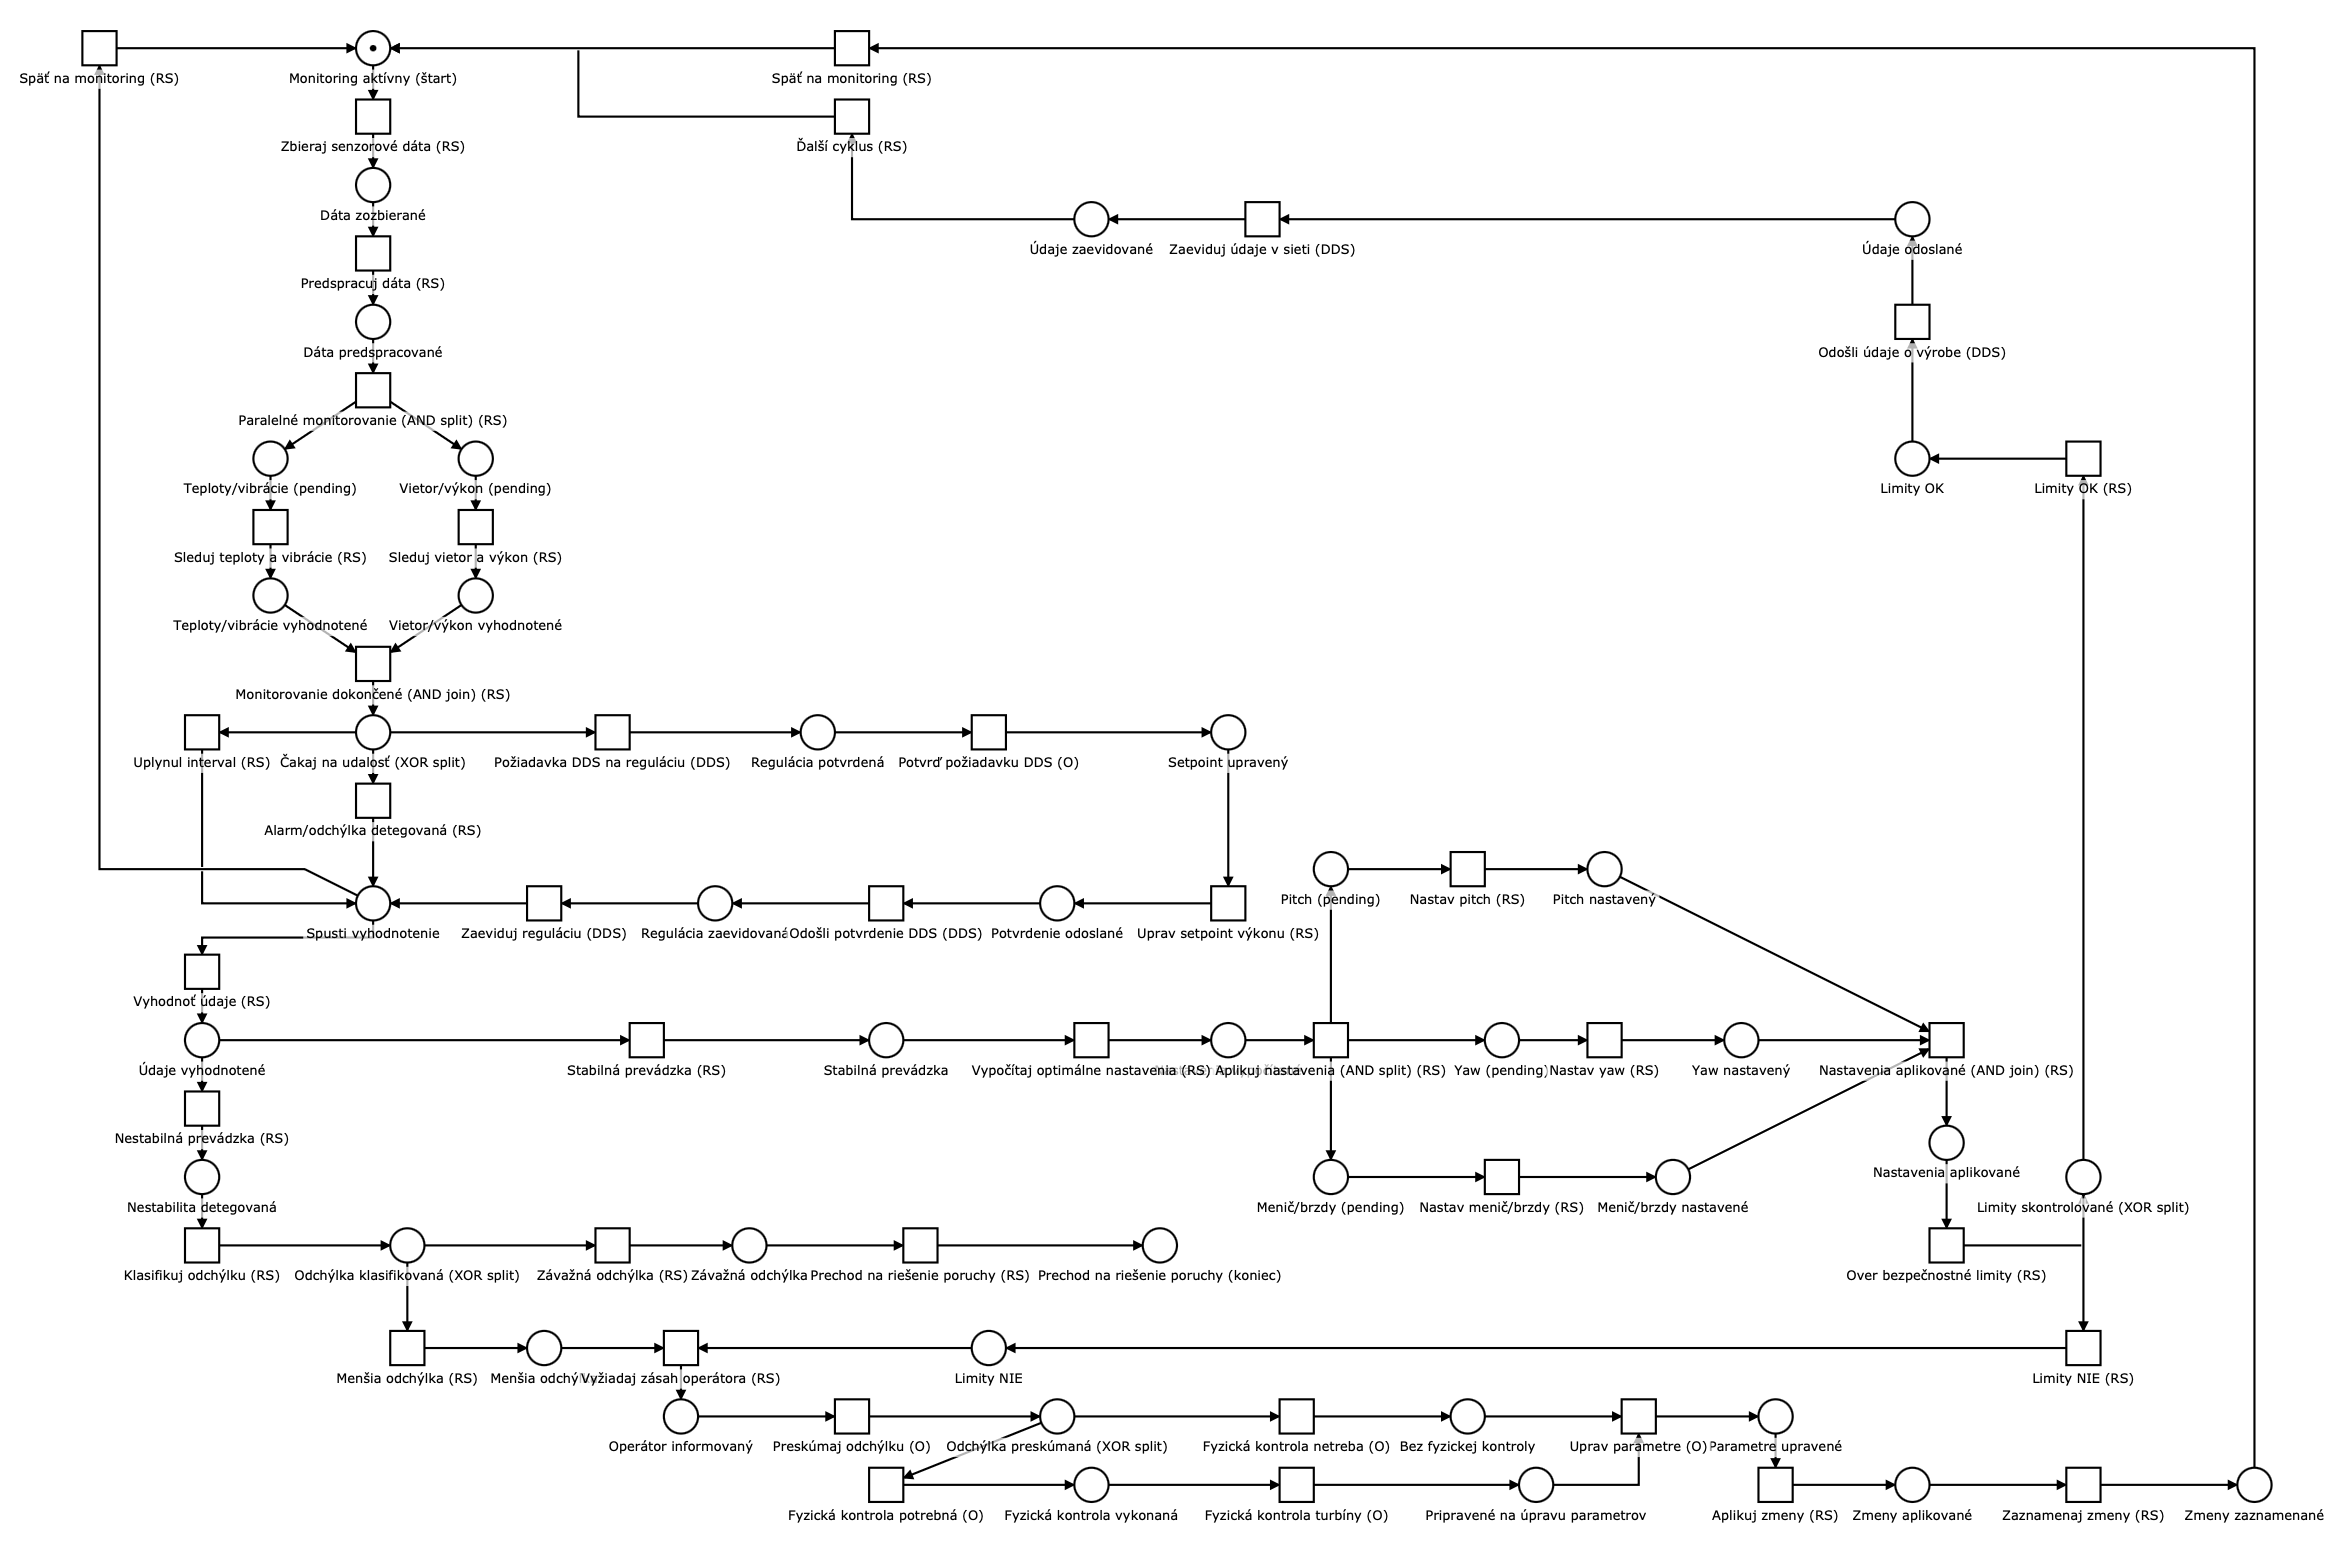
\includegraphics[width=\textwidth]{figs/P2/PS_P2.png}
  \caption{Petriho sieť pre Proces 2}
\end{figure}


%%%%%%%%%%%%%%%%%%%%%%%%%%%%%%%%%%%%%%%%%%%%%%%%%%%%%%%%%%%%%%
%Reachability grapah
%%%%%%%%%%%%%%%%%%%%%%%%%%%%%%%%%%%%%%%%%%%%%%%%%%%%%%%%%%%%%%
\newpage
\subsection{Graf dosiahnuteľnosti}
\begin{figure}[H]
  \centering
  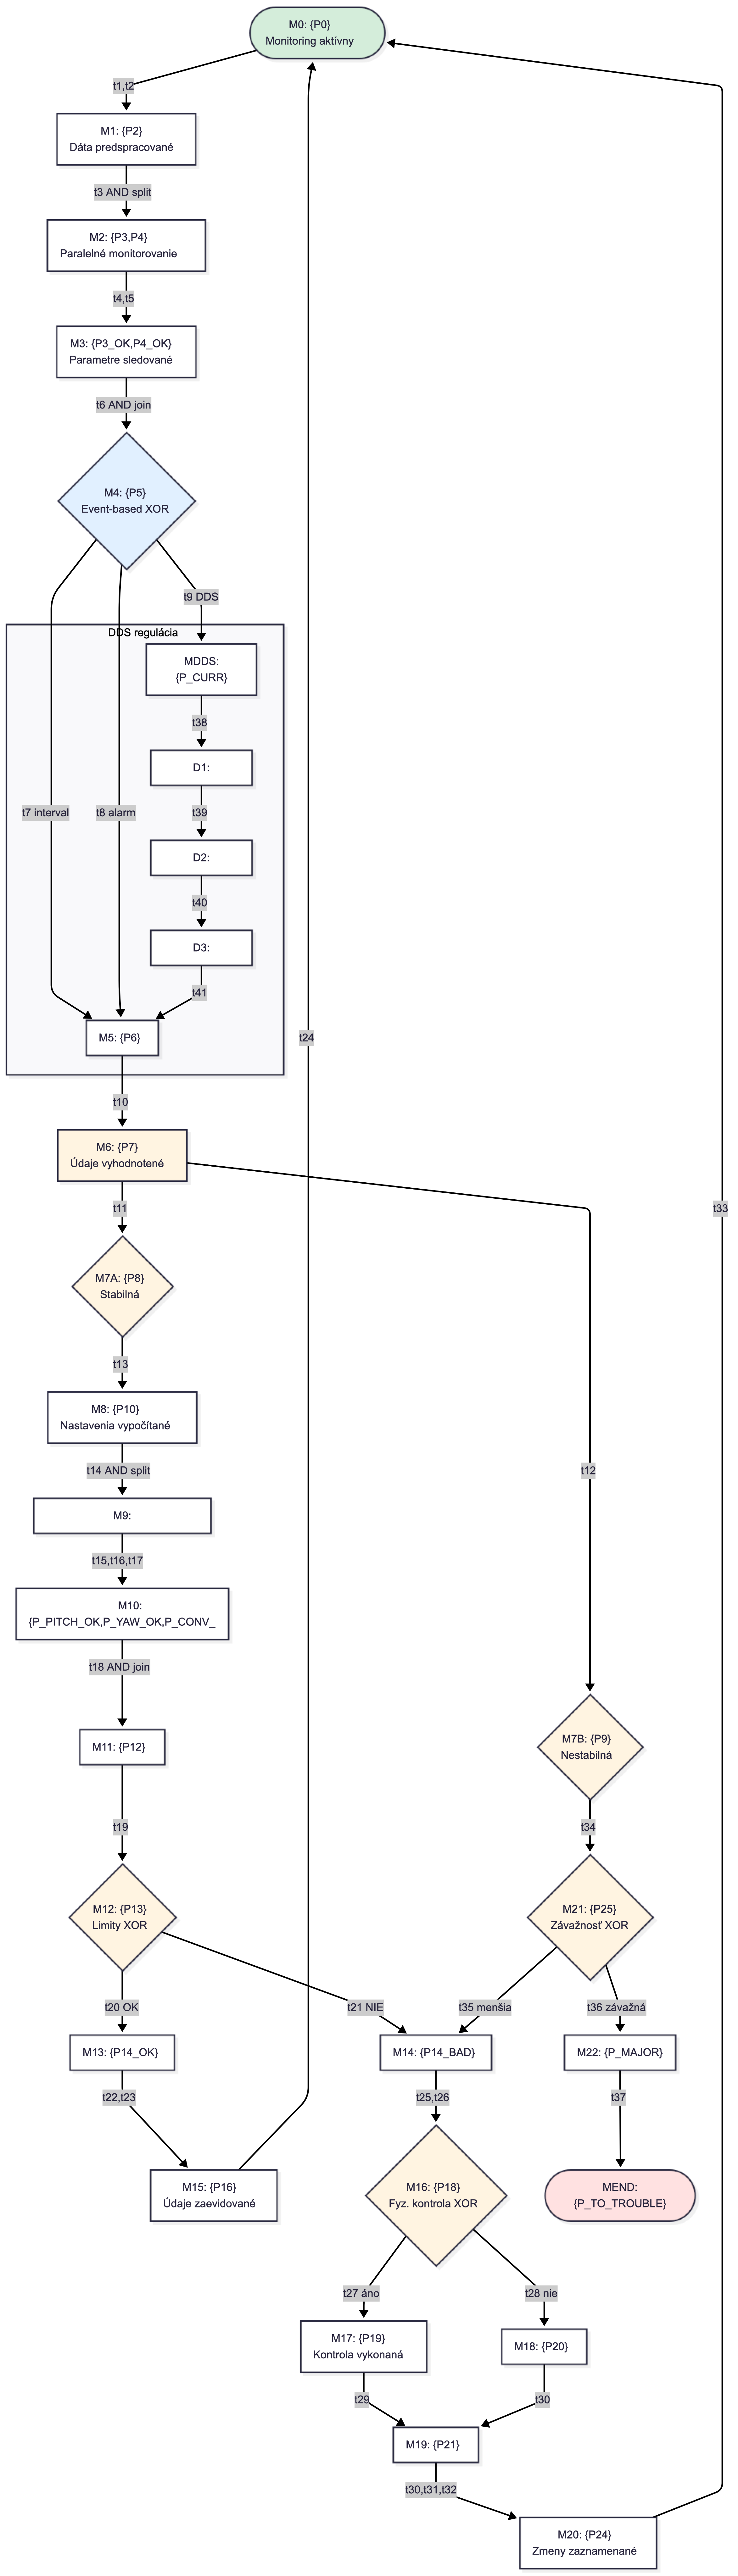
\includegraphics[height=0.9\textheight]{figs/P2/P2_ReachabilityGraph.png}
  \caption{Proces 2 -- Graf dosiahnuteľnosti}
\end{figure}

%%%%%%%%%%%%%%%%%%%%%%%%%%%%%%%%%%%%%%%%%%%%%%%%%%%%%%%%%%%%%%
%Screens
%%%%%%%%%%%%%%%%%%%%%%%%%%%%%%%%%%%%%%%%%%%%%%%%%%%%%%%%%%%%%%
\newpage
\subsection{Obrazovky}
\emph{TODO: Doplniť}

%%%%%%%%%%%%%%%%%%%%%%%%%%%%%%%%%%%%%%%%%%%%%%%%%%%%%%%%%%%%%%
%BPMN
%%%%%%%%%%%%%%%%%%%%%%%%%%%%%%%%%%%%%%%%%%%%%%%%%%%%%%%%%%%%%%
\newpage
\subsection{BPMN}
\begin{figure}[H]
  \centering
  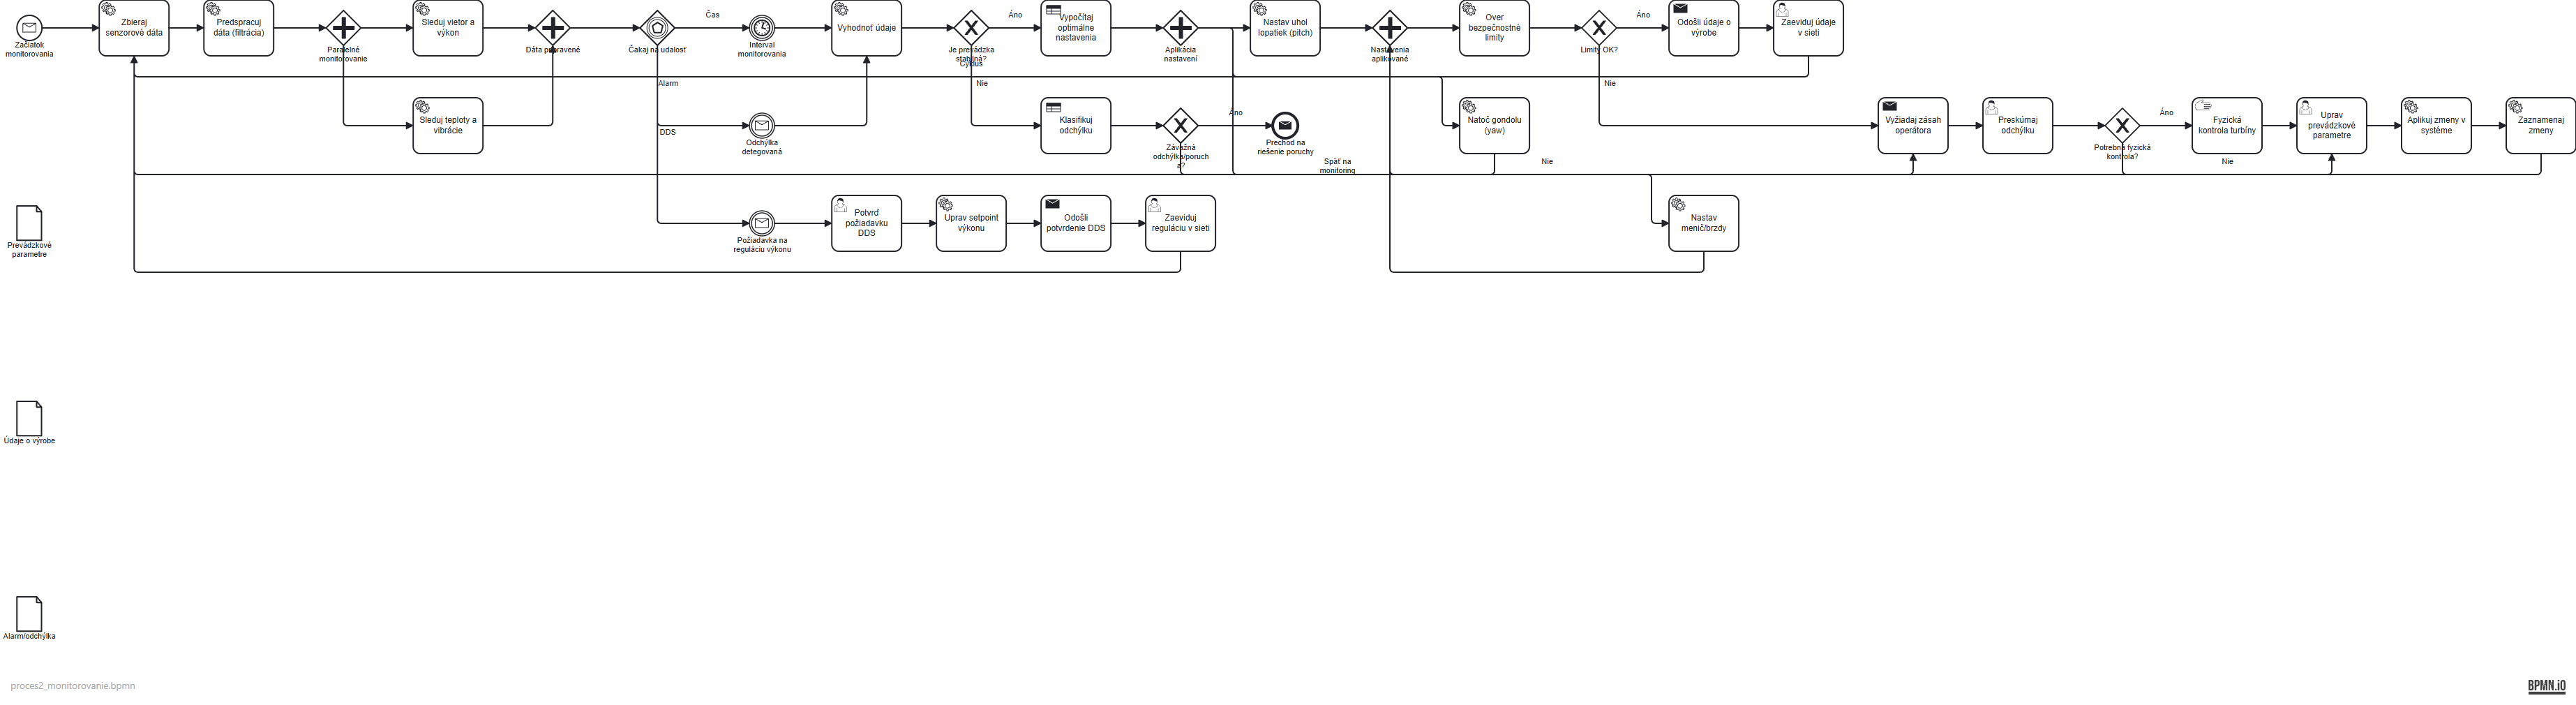
\includegraphics[width=\textwidth]{figs/P2/proces2-monitorovanie.png}
  \caption{Proces 2 -- BPMN model}
\end{figure}




%%%%%%%%%%%%%%%%%%%%%%%%%%%%%%%%%%%%%%%%%%%%%%%%%%%%%%%%%%%%%%
%P3
%%%%%%%%%%%%%%%%%%%%%%%%%%%%%%%%%%%%%%%%%%%%%%%%%%%%%%%%%%%%%%
\newpage
\section{Proces 3 -- Riešenie poruchy a obnovenie prevádzky}
\subsection{Popis procesu}
Proces riešenia poruchy začína zaznamenaním poruchového hlásenia. Poruchu najskôr deteguje riadiaci systém, ktorý zároveň zaznamená hlásenie o vzniknutej poruche. Následne operátor elektrárne vyhodnotí situáciu a rozhoduje, či ide o kritickú poruchu. Ak ide o kritickú poruchu, riadiaci systém vykoná núdzové zastavenie turbíny. Ak porucha nie je kritická, operátor zabezpečí plánované odstavenie zariadenia.

Po odstavení zariadenia sa riadiacim systémom vytvorí servisná úloha, na základe ktorej servisný technik vykoná diagnostiku problému a následne realizuje opravu. Po dokončení opravy servisný technik vykoná test funkčnosti zariadenia. Na základe výsledku testu sa rozhodne, či je zariadenie v poriadku. Ak je zariadenie funkčné, riadiaci systém zabezpečí opätovné spustenie výroby a dispečer distribučnej siete je informovaný o obnovení dodávky. Proces sa tým končí obnovením prevádzky. Ak zariadenie nie je v poriadku, problém sa eskaluje a proces riešenia sa opakuje až do úspešného odstránenia poruchy alebo odovzdania problému na vyššiu úroveň riešenia.
Ak oprava trvá neprimerane dlho, operátor elektrárne eskaluje problém (napr. na vyššiu úroveň podpory).

\subsection{Procesné informácie (tokeny, prechody, stavy)}
\begin{table}[H]
  \centering
  \renewcommand{\arraystretch}{1.2}
  \begin{tabularx}{\textwidth}{|p{0.22\textwidth}|X|}
    \hline
    \textbf{Názov procesu} & Riešenie poruchy a obnovenie prevádzky \\
    \hline
    \textbf{Popis} & Po detekcii poruchy systém zaznamená hlásenie, zhromaždí diagnostické údaje a operátor rozhodne o kritickosti. Pri kritickej poruche prebehne núdzové zastavenie, inak plánované odstavenie. Po odstavení sa paralelne vytvorí servisná úloha, informuje sa dispečer a zabezpečí sa prístup a bezpečnosť na mieste. Servisný technik vykoná diagnostiku a opravu; ak je potrebný náhradný diel, čaká sa na dodávku a rieši sa oneskorenie. Po úspešnej oprave systém požiada DDS o opätovné pripojenie (schválenie/zamietnutie/timeout) a po schválení obnoví výrobu a odošle oznámenie, ktoré DDS zaeviduje. Pri dlhom riešení môže operátor incident eskalovať. \\
    \hline
    \textbf{Roly} & Riadiaci systém (RS), Operátor elektrárne (O), Servisný technik (ST), Dispečer distribučnej siete (DDS) \\
    \hline
    \textbf{Vstupné tokeny} & Poruchové hlásenie (alarm), diagnostické údaje, servisná požiadavka, dostupnosť pripojenia do siete (DDS), náhradné diely \\
    \hline
    \textbf{Výstupné tokeny} & Prevádzka obnovená + zaevidovanie v DDS alebo eskalovaný incident / odložené pripojenie (opakovaná žiadosť) \\
    \hline
    \textbf{Prechody} & Deteguj poruchu, zaznamenaj hlásenie, zhromaždi diagnostické údaje, vyhodnoť situáciu, rozhodni kritickosť, núdzové zastavenie / plánované odstavenie, vytvor servisnú úlohu, informuj DDS o odstávke, zaeviduj odstávku, zabezpeč prístup, diagnostika na mieste, čakanie na diel / urgencia, výmena dielu, oprava/kalibrácia, test funkčnosti, rozhodni či je zariadenie OK, požiadaj o opätovné pripojenie, čakaj na odpoveď DDS, naplánuj opätovnú žiadosť / kontaktuj DDS, opätovne spusti výrobu, odošli oznámenie o obnovení, zaeviduj obnovu, eskaluj problém \\
    \hline
    \textbf{Stavy} & Porucha detegovaná, hlásenie zaznamenané, diagnostické údaje pripravené, turbína odstavená, servisná úloha vytvorená, DDS informovaná, odstávka zaevidovaná, prístup zabezpečený, diagnostika vykonaná, diel potrebný/nepotrebný, diel doručený/oneskorený, oprava vykonaná, test vykonaný, zariadenie OK/nie OK, žiadosť o pripojenie odoslaná, odpoveď DDS prijatá (schválené/zamietnuté/timeout), výroba obnovená, obnova zaevidovaná, incident eskalovaný \\
    \hline
  \end{tabularx}
  \caption{Proces 3 -- Zhrnutie procesu}
\end{table}

\subsection{Procesné roly}
\begin{table}[H]
  \centering
  \renewcommand{\arraystretch}{1.2}
  \begin{tabularx}{\textwidth}{|p{0.22\textwidth}|X|}
    \hline
    \textbf{Rola} & \textbf{Úloha} \\
    \hline
    Riadiaci systém & Deteguje poruchu, zaznamenáva hlásenia, zhromažďuje diagnostické údaje, vykonáva núdzové zastavenie (ak treba), vytvára servisnú úlohu, informuje DDS, žiada o opätovné pripojenie a po schválení zabezpečuje obnovenie výroby a odoslanie oznámenia. \\
    \hline
    Operátor elektrárne & Vyhodnocuje situáciu, rozhoduje o kritickosti poruchy a o type odstavenia; zabezpečuje prístup a bezpečnosť, pri zamietnutí/timeoutoch koordinuje opakovanú žiadosť a pri dlhom riešení eskaluje incident. \\
    \hline
    Servisný technik & Vykonáva diagnostiku na mieste, realizuje opravu/kalibráciu a test funkčnosti; ak je potrebný náhradný diel, rieši čakanie a výmenu dielu, následne rozhoduje o pripravenosti zariadenia na spustenie. \\
    \hline
    Dispečer distribučnej siete & Eviduje odstávku a obnovu dodávky v sieti a poskytuje odpoveď na žiadosť o opätovné pripojenie (schválenie/zamietnutie). \\
    \hline
  \end{tabularx}
  \caption{Proces 3 -- Popis rolí}
\end{table}

\subsection{Procesné roly (priradenie činností)}
\begin{table}[H]
  \centering
  \small
  \renewcommand{\arraystretch}{1.2}
  \begin{tabularx}{\textwidth}{|X|p{0.14\textwidth}|p{0.14\textwidth}|p{0.14\textwidth}|p{0.14\textwidth}|}
    \hline
    \textbf{Činnosť} & \textbf{RS} & \textbf{O} & \textbf{ST} & \textbf{DDS} \\
    \hline
    Deteguj poruchu & X &  &  &  \\
    \hline
    Zaznamenaj hlásenie & X &  &  &  \\
    \hline
    Zhromaždi diagnostické údaje & X &  &  &  \\
    \hline
    Vyhodnoť situáciu &  & X &  &  \\
    \hline
    Rozhodni kritickosť poruchy &  & X &  &  \\
    \hline
    Núdzové zastavenie turbíny & X &  &  &  \\
    \hline
    Plánované odstavenie &  & X &  &  \\
    \hline
    Vytvor servisnú úlohu & X &  &  &  \\
    \hline
    Informuj DDS o odstávke & X &  &  &  \\
    \hline
    Zaeviduj odstávku v sieti &  &  &  & X \\
    \hline
    Zabezpeč prístup a bezpečnosť &  & X &  &  \\
    \hline
    Diagnostika na mieste &  &  & X &  \\
    \hline
    Urgencia dodávky dielu &  &  & X &  \\
    \hline
    Vymeň náhradný diel &  &  & X &  \\
    \hline
    Oprava/kalibrácia &  &  & X &  \\
    \hline
    Test funkčnosti zariadenia &  &  & X &  \\
    \hline
    Rozhodni či je zariadenie OK &  &  & X &  \\
    \hline
    Požiadaj o opätovné pripojenie & X &  &  &  \\
    \hline
    Naplánuj opätovnú žiadosť &  & X &  &  \\
    \hline
    Kontaktuj DDS &  & X &  &  \\
    \hline
    Opätovne spusti výrobu & X &  &  &  \\
    \hline
    Odošli oznámenie o obnovení & X &  &  &  \\
    \hline
    Zaeviduj obnovu dodávky &  &  &  & X \\
    \hline
    Eskaluj problém &  & X &  &  \\
    \hline
  \end{tabularx}
  \caption{Proces 3 -- Priradenie činností k rolám}
\end{table}

\subsection{Petriho sieť}
Model procesu bol navrhnutý ako Petriho sieť v nástroji Netgrif Builder. Model obsahuje rozhodovanie (XOR split), paralelné vetvenie (AND split), dátové polia (enumeration\_map) a TaskRef na úlohu z iného procesu.
\begin{figure}[H]
  \centering
  
\includegraphics[width=\textwidth]{petri/proces3-porucha.png}
  \caption{Proces 3 -- Petriho sieť}
\end{figure}

\subsection{Graf dosiahnuteľnosti}
\emph{TODO: Sem doplniť graf dosiahnuteľnosti pre vybraný proces.}

\subsection{Obrazovky}
\emph{TODO: Sem doplniť návrh obrazoviek pre prechody Petriho siete.}

\subsection{BPMN}
\begin{figure}[H]
  \centering
  
\includegraphics[width=\textwidth]{bpmn/proces3-porucha.png}
  \caption{Proces 3 -- BPMN model}
\end{figure}

\section{Poznámky k súladu so zadaním}
\begin{itemize}
  \item Slovné popisy: v dokumente sú popísané 3 procesy (splnené).
  \item Procesné roly: v dokumente sú tabuľky rolí a činností pri každom procese; celkovo sú identifikované minimálne 4 roly (splnené).
  \item BPMN: doplnené AND/XOR brány, event-based brána, cyklus, podproces, boundary event a artefakty (splnené).
  \item Petriho siete: doplnené obrázky modelov procesov (splnené).
  \item Grafy dosiahnuteľnosti a obrazovky: ponechané ako TODO (doplní sa v ďalšom kroku).
\end{itemize}

\end{document}